\subsection{旋转法构建端盖三维模型}
\begin{procedure}
\item 切换西南等轴测图

\item 旋转构建端盖三维模型
旋转产生$\phi 9$圆柱体。
\begin{lstlisting}
|命令: revolve|
|当前线框密度:  ISOLINES=4,闭合轮廓创建模式 = 实体|
|选择要旋转的对象或 [模式(MO)]: MO 闭合轮廓创建模式 [实|
|体(SO)/曲面(SU)] $<$实体$>$: SO|
|选择要旋转的对象或 [模式(MO)]: 找到 1 个|
|选择要旋转的对象或 [模式(MO)]:|
|指定轴起点或根据以下选项之一定义轴 [对象(O)/X/Y/Z] $<$对象$>$:|
|指定轴端点:|
|指定旋转角度或 [起点角度(ST)/反转(R)/表达式(EX)] $<$360$>$:|
\end{lstlisting}
旋转产生端盖主特征三维模型,其结果如图\ref{fig:duangai1}所示。

\begin{lstlisting}
|命令: revolve|
|当前线框密度:  ISOLINES=4,闭合轮廓创建模式 = 实体|
|选择要旋转的对象或 [模式(MO)]: MO 闭合轮廓创建模式 [实|
|体(SO)/曲面(SU)] $<$实体$>$: SO|
|选择要旋转的对象或 [模式(MO)]: 找到 1 个|
|选择要旋转的对象或 [模式(MO)]:|
|指定轴起点或根据以下选项之一定义轴 [对象(O)/X/Y/Z] $<$对象$>$:|
|指定轴端点:near 到|
|指定旋转角度或 [起点角度(ST)/反转(R)/表达式(EX)] $<$360$>$:|
\end{lstlisting}
\item 三维阵列$\phi 9$圆柱体,其结果如图\ref{fig:duangai2}所示。
\begin{lstlisting}
|命令: 3darray|
|选择对象: 找到 1 个|
|选择对象:|
|输入阵列类型 [矩形(R)/环形(P)]$<$矩形$>$:p|
|输入阵列中的项目数目: 6|
|指定要填充的角度 (+=逆时针, -=顺时针)$ <360>$:|
|旋转阵列对象? [是(Y)/否(N)] $<Y>$:|
|指定阵列的中心点:|
|指定旋转轴上的第二点:|
\end{lstlisting}
\begin{figure}[htbp]
\centering
\subfloat[]{\label{fig:duangai1}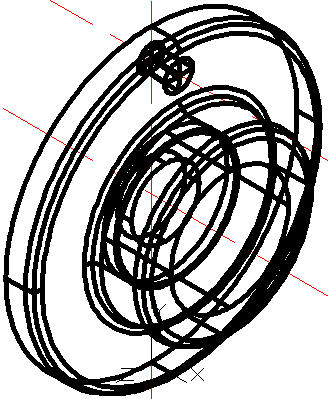
\includegraphics[scale=0.45]{duangai1.png}}\hspace{30pt}
\subfloat[]{\label{fig:duangai2}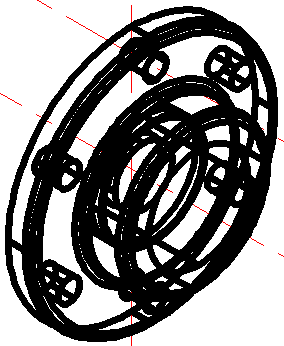
\includegraphics[scale=0.5]{duangai2.png}}\hspace{30pt}
\subfloat[]{\label{fig:duangailititu}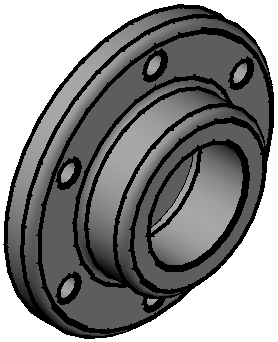
\includegraphics[scale=0.5]{duangailititu.png}}
\caption{端盖三维模型构建过程}
\end{figure}
\item 用差集操作完成三维建模操作。
\begin{lstlisting}
|命令: subtract |
|选择要从中减去的实体、曲面和面域...|
|选择对象: 找到 1 个|
|选择对象:  选择要减去的实体、曲面和面域...|
|选择对象: 找到 1 个|
|选择对象: 找到 1 个,总计 2 个|
|选择对象: 找到 1 个,总计 3 个|
|选择对象: 找到 1 个,总计 4 个|
|选择对象: 找到 1 个,总计 5 个|
|选择对象: 找到 1 个,总计 6 个|
|选择对象:|
\end{lstlisting}
\item 设置视觉样式为真实,其结果如图\ref{fig:duangailititu}所示。
\item 将端盖模型保存为“调压阀端盖立体图.dwg”。
\end{procedure}